
\chapter{\label{chapter3_EHT}A regulatory network model underlying the endothelial-to-haematopoietic transition}
\chaptermark{Chapter 3 - EHT GRN}

\begingroup
\raggedright
\minitoc
\endgroup

\clearpage % Keep contents seperate page

\section{Introduction and aims}

EHT is an essential process for the initial formation of the haematopoietic system. It involves the specification of endothelial cells into haemogenic endothelium and differentiation into HSCs and haematopoietic progenitor cells (HPCs) \citep{bertrand_haematopoietic_2010, boisset_vivo_2010, kissa_blood_2010}. EHT involves cell differentiation through several distinct intermediates, extensive morphological changes, and genome wide transcriptional changes. Exploring how the transcriptome is regulated during EHT is essential for understanding what drives this process. Additionally, the well-defined cell types and dynamic transcription offers this system as an ideal model to explore the activity of TFs, and how these regulators drive specific processes and cell-type transitions underlying EHT. 

It is well established that Runx1 is a master regulator critical for EHT \citep{cai_haploinsufficiency_2000, chen_runx1_2009, north_cbfa2_1999}. It is therefore important to understand the context of Runx1 within the EHT process, such as its key upstream regulators and downstream targets. TFs do not act in isolation, and commonly function together. For example, Runx1 is known to cooperate with many different TFs, such as PU.1 and Ets1 \citep{kim_mutual_1999, goetz_auto-inhibition_2000, hu_runx1_2011}, and can alter the DNA binding preference of other factors as with Fli1 \citep{lichtinger_runx1_2012}. More recently, in T-cell development Runx1 has been found to cooperate with Gata3 to drive a silencer for \textit{Spi1} \citep{hosokawa_stage-specific_2021}, and to cooperate with Runx3 to additively regulate gene expression with high functional redundancy \citep{shin_runx1_2021}. Exploring how Runx1 cooperates with other TFs will offer both greater understanding of EHT, as well as insight into which other TFs cooperate to drive gene expression. 

To explore the regulation of EHT in this chapter, I have constructed a GRN model integrating RNA-seq and ATAC-seq data. A GRN model is an ideal method to interrogate this system, as it allows us to determine the key drivers of specific processes, as well as to explore the combinatorial logic of TFs functioning cooperatively. Several studies have attempted to characterise the regulatory network underpinning EHT \citep{goode_dynamic_2016, baron_single-cell_2018, zhu_developmental_2020, zeng_tracing_2019, bergiers_single-cell_2018, gao_transcriptional_2020}, however these studies have primarily focused on E10.5 and E11.5 mouse embryos and have not investigated E8.5 mouse embryos where HE signals are first received. As such, the initial transcriptional changes occurring in early-EHT intermediates have been poorly studied, and lack characterisation of the E8.5 pre-HE population. In this chapter I aimed to construct a GRN model incorporating both early (pre-HE) and late (pre-HSC) populations, covering the full range of EHT intermediates.

\noindent
\textbf{Aims}
 
\vspace*{-5mm}
\begin{enumerate}
    \item Establish a GRN describing early and late endothelial-to-haematopoietic transition. 
    \item Profile regulators of \textit{Runx1} and downstream targets. 
    \item Investigate transcription factor cooperativity that drives haematopoietic processes. 
\end{enumerate}

\vspace*{-5mm}
By constructing a GRN describing both early and late EHT, and profiling the regulators of Runx1, this analysis will improve our understanding of how EHT is initiated in the early stages of HE specification. Investigating TF cooperativity, will allow us to explore a less understood aspect of gene regulation that may be important in driving key processes.

\clearpage

\section[Profiling of EHT sub-populations reveals dynamic transcription and chromatin accessibility changes]{\label{ch3:overview}Profiling of EHT sub-populations reveals\\dynamic transcription and chromatin\\accessibility changes}

To probe EHT in detail the de Bruijn lab uses a \textit{Runx1} +23 enhancer GFP reporter (23GFP) mouse model \citep{bee_nonredundant_2010}, with specific activity in HE and IACs, allowing us to dissect early stages of EHT. 23GFP activity marks HE (Fig. \ref{fig:ch3_overview}A), and can be used to label a pre-HE population in E8.5 dorsal aorta endothelium that precedes active \textit{Runx1} transcription \citep{swiers_early_2013}. This early activation of the +23 enhancer implies early regulatory signals prior to the onset of endogenous \textit{Runx1} expression and EHT. As such, by using the 23GFP mouse model, HE can be isolated from E9.5 embryos and pre-HE can be isolated from E8.5 embryos, with a key difference between these populations being the detection of endogenous \textit{Runx1} transcripts (Fig. \ref{fig:ch3_overview}A, \cite{swiers_early_2013}).

\begin{figure}[!b]
    \centering
    \includegraphics[width=\textwidth,height=\textheight,keepaspectratio]{figures/chapter3/ch3_overview.png}
    \caption[{Overview of profiled EHT populations.}]
    {\textbf{Overview of profiled EHT populations.} 
    \textbf{(A)} Top – Schematic of the \textit{Runx1} locus, with the +23 enhancer annotated in green. Bottom –  Immunofluorescence image of whole-mount 23GFP E10.5 AGM, showing a single 2.5 $\mu$m slice. 23GFP marked HE and IACs. 
    \textbf{(B)} Schematic of EHT cell populations sorted from E8.5, E9.5 and E10.5 mouse embryos, that were profiled by RNA-seq and ATAC-seq. Bars indicate population sort markers. Populations were first gated on Ter119\uneg{}. RNA-seq \textit{n} = 3 (pre-HE = 4) and ATAC-seq \textit{n} = 4 (pro-HSC = 3). 
    \textit{RNA-seq and ATAC-seq data were generated by previous members of the de Bruijn lab (G. Swiers and L.Greder, respectively) and were used in analyses and GRN construction performed by me.}
    }
    \label{fig:ch3_overview}
\end{figure}

To investigate the regulatory logic driving EHT I used data generated previously in the de Bruijn lab, namely transcription profiling and chromatin accessibility of bulk populations from the PAS/AGM + VU of E8.5 to E10.5 mouse embryos (Fig. \ref{fig:ch3_overview}B, Appendix \ref{fig:app_eht-sort-gates}A). These populations include E8.5 endothelial cells (EC, Ter119\uneg{}VECad\upos{}CD41\uneg{}CD45\uneg{}23GFP\uneg{}) and pre-HE (Ter119\uneg{}VECad\upos{}CD41\uneg{}CD45\uneg{}23GFP\upos{}), E9.5 HE (Ter119\uneg{}VECad\upos{}\-CD41\uneg{}CD45\uneg{}23GFP\upos{}) and pro-HSC (Ter119\uneg{}VECad\upos{}CD41\upos{}CD45\uneg{}), and E10.5 pre-HSC I (Ter119\uneg{}VECad\upos{}\-CD41\upos{}CD45\uneg{}) and pre-HSC II (Ter119\uneg{}VECad\upos{}CD41\upos{}CD45\upos{}). Sort panels for these populations did not include CD43, so the population indicated as 'pro-HSC' contains both pro-HSC (CD43\uneg{}, \cite{rybtsov_tracing_2014}) and blood progenitors (CD43\upos{}). E9.5 Ter119\uneg{}VECad\upos{}CD41\upos{}CD45\uneg{} PAS cells contain 80.3 \textpm 4.8\% CD43\upos{} haematopoietic progenitors (Appendix \ref{fig:app_eht-sort-gates}B).

Following pre-processing and mapping, reads were found to have high levels of PCR duplication (RNA-seq: 28\% - 72.7\% PCR duplication, with mean of 49.5\%. ATAC-seq: 58.3\% - 89\% PCR duplication, with mean of 78.5\%), and after PCR duplicate removal mapping was successful (Appendix \ref{fig:app_eht-qc}). Low-expressing genes were removed from the RNA-seq data (see methods section \ref{ch2:rna-analysis}, p.\pageref{ch2:rna-analysis}), before pre-processing with EdgeR \citep{robinson_edger:_2010}. Peak-calls were generated from individual ATAC-seq samples, and peaks overlapping in at least two replicates were retained, in order to discard low-quality peak calls. ATAC-seq signal was quantified over these robust peaks to create a peak read count table, and as with the RNA-seq data low count peaks were discarded (see methods section \ref{ch2:chip-atac-analysis}, p.\pageref{ch2:chip-atac-analysis}). 

\subsection[Different EHT expression signatures drive differentiation, morphological, and signalling processes]{\label{ch3:profiling}Different EHT expression signatures drive\\differentiation, morphological, and signalling\\processes}

\begin{figure}[!b]
    \centering
    \includegraphics[width=\textwidth,height=\textheight,keepaspectratio]{figures/chapter3/ch3_pca.png}
    \caption[{EHT principal components define switch and transient gene regulation.}]
    {\textbf{EHT principal components define switch and transient gene regulation.} 
    \textbf{(A)} PCA plots of RNA-seq (left) and ATAC-seq (right) samples that describe the EHT transition. ANOVA DEG and DAEs used as input. 
    \textbf{(B)} Heatmap of RNA-seq gene expression (Log\textsubscript{2} CPM) ordered by PCA loading contribution to PC1 (left) and PC2 (right).
    \textbf{(C)} Top PC1+, PC1-, and PC2+ loadings relating to the RNA-seq PCA shown in A-B.
    \textbf{(D)} Average gene expression (CPM) plots for strong PC1 and PC2 loading genes. Error bars represent standard error of the mean; \textit{n} = 3; \textit{n} = 4 for pre-HE.
    }
    \label{fig:ch3_pca}
\end{figure}

To explore gene regulation in EHT, I first analysed general gene expression and chromatin accessibility profiles. As pairwise analysis between populations does not incorporate changes across the whole EHT process, I instead performed an ANOVA-like test in EdgeR \citep{robinson_edger:_2010} to extract differentially expressed genes (DEGs) from the RNA-seq data, and differentially accessible elements (DAEs) from the ATAC-seq data. This method tests for changes between any populations, and therefore identifies gene expression and ATAC accessibility generally associated with EHT. ANOVA tests identified 5892 DEGs in the RNA-seq data, and 17969 DAEs in the ATAC-seq data. 

PCA of the DEGs and DAEs clustered replicates together (Fig. \ref{fig:ch3_pca}A). The PC1 axis in both RNA-seq and ATAC-seq datasets represents a sequential progression of EHT. PC2 instead describes a transient activation or suppression of transcription, where expression peaks or troughs in HE/pro-HSC and returns to baseline levels in pre-HSCs (Fig. \ref{fig:ch3_pca}B). For example, \textit{Lin28a} is PC1- associated with high EC expression and is known to negatively regulate haematopoiesis \citep{chaudhuri_oncomir_2012}, while \textit{Gpr56} is PC1+ associated with high pre-HSC expression and is required for HSC generation \citep{solaimani_kartalaei_whole-transcriptome_2015} (Fig. \ref{fig:ch3_pca}C-D). \textit{Igfbp3} is PC2+ associated and transiently regulated with peak expression in HE (Fig. \ref{fig:ch3_pca}C-D), and is implicated in a range of pathways \citep{baxter_insulin-like_2013} but has not previously been implicated in EHT. PC1 loadings can be considered to reflect genes that switch on or off, while PC2 loadings represent transient regulation.

To properly categorise these DEGs and DAEs into different patterns, the RNA-seq and ATAC-seq counts were clustered into five regulatory modules (RNA1-5 and ATAC1-5, Fig. \ref{fig:ch3_clusters}A-B). The modules represent transient decrease (RNA1/ATAC1) or increase (RNA3/ATAC3) in RNA-seq and ATAC-seq counts, an endothelial bias (RNA2/ATAC2), early haematopoietic commitment (upregulation in HE/pro-HSC, RNA4/ATAC4), and late haematopoietic commitment (upregulation in pre-HSC I/II, RNA5/ATAC5). It is striking that similar patterns are observed between RNA-seq and ATAC-seq datasets. Clusters have been labelled to represent similar patterns between the datasets, such as RNA2 and ATAC2, both of which are downregulated over EHT. 

\begin{figure}[htbp]
    \centering
    \includegraphics[width=\textwidth,height=\textheight,keepaspectratio]{figures/chapter3/ch3_clusters.png}
    \caption[{Transient regulation activates signalling and morphological changes while switches drive a haematopoietic phenotype.}]
    {\textbf{Transient regulation activates signalling and morphological changes while switches drive a haematopoietic phenotype.} 
    \textbf{(A)} Expression and accessibility heatmaps (Z-score Log\textsubscript{2} CPM) for RNA-seq DEGs  (left) and ATAC-seq DAEs (right). Expression grouped by hierarchical clustering, and accessibility by \textit{k}-means clustering. 
    \textbf{(B)} Average z-score Log\textsubscript{2} CPM of gene expression (left), or chromatin accessibility (right) by clusters as in A. Fishers exact test results comparing the overlap of corresponding RNA- and ATAC-seq clusters are shown on the side. 
    \textbf{(C-D)} GO biological process enrichment for modules RNA1-5 (C) and ATAC1-5 (D). Only significant data points shown (P $\leq$ 0.05).
    }
    \label{fig:ch3_clusters}
\end{figure}

As enhancer and promoter activity should drive gene expression changes it is expected that ATAC-seq peaks would be associated with genes within the same module, such as ATAC2 accessible elements linked to RNA2 genes. To test this hypothesis, I annotated each DAE to the closest DEG to associate enhancer and promoter elements to the corresponding gene. I then performed Fisher's exact tests to determine the significance of overlap between genes in RNA1-5 and genes linked to accessible elements in corresponding ATAC1-5 modules (Fig. \ref{fig:ch3_clusters}B). Each corresponding RNA-seq and ATAC-seq module, other than RNA1 and ATAC1, was significantly associated with each other, supporting the hypothesis that differential enhancer and promoter accessibility is driving gene expression changes.

These modules describe a range of dynamic profiles across EHT, though it is unclear whether clustering the data has functional relevance. To determine whether these modules drive specific programs, I performed gene ontology (GO) enrichment analyses (Fig. \ref{fig:ch3_clusters}C-D). Transiently activated genes (RNA3/ATAC3) are associated with Notch and BMP signalling, and processes that underpin morphological changes and migration, including epithelial-to-mesenchyme transition (EMT) and actin cytoskeleton organisation (Fig. \ref{fig:ch3_clusters}C-D). Late haematopoietic commitment (RNA5/ATAC5) is instead enriched for terms related to cytokine production, haematopoiesis, and T cell activation, corresponding with a differentiation program. This breakdown of regulatory patterns highlights the complex regulation over EHT and begins to categorise distinct regulatory programs. In particular, transient activation is associated with signalling and morphological changes that may drive the budding process during EHT.

\subsection{\label{ch3:cd109}Transition-specific regulation}

EHT is controlled through specific sequential transitions between cell types. Therefore, an initial characterisation of RNA-seq and ATAC-seq changes at these transitions is important to understand. In particular, understanding the difference between E8.5 ECs and E8.5 pre-HE can identify key genes that distinguish this pre-HE population. To identify specific regulatory changes characterising cell type transitions I performed pairwise differential analyses between sequential EHT populations. As with the ANOVA analysis, DAEs were associated with the closest DEG promoter. As it is expected for changes in chromatin accessibility to reflect gene expression, I examined the relationship between RNA-seq and ATAC-seq logFC between transitions. Changes in chromatin accessibility and gene expression are generally concordant, such as with the EC to pre-HE transition where 79\% of opening chromatin elements associate with upregulated genes (Fig. \ref{fig:ch3_stage-enhs}A). This concordance is not present in all transitions, such as the pre-HE to HE transition where 33\% of closing elements are associated with increasing expression (Fig. \ref{fig:ch3_stage-enhs}A). This could be due to incorrect assignment of elements to gene promoters, or reflect silencers or non-regulatory elements.

\begin{figure}[t]
    \centering
    \includegraphics[width=\textwidth,height=\textheight,keepaspectratio]{figures/chapter3/ch3_stage-enhs.png}
    \caption[{Analysis of enhancer-promoter pairs suggests stage-specific epigenetic regulation.}]
    {\textbf{Analysis of enhancer-promoter pairs suggests stage-specific epigenetic regulation.} 
    \textbf{(A)} Relationship between RNA- and ATAC-seq logFC at significant pairwise comparisons. Each data point represents an accessible element paired with a gene (as defined by closest DEG promoter to the element). Only non-promoter elements are shown (distance > 1kb from TSS). High logFC genes that have relevance to EHT based on existing literature were highlighted red, and examined in B.  
    \textbf{(B)} ATAC-seq tracks for DAEs, as highlighted in A. Sample replicates were combined into a single track. Values indicate track height. Opening elements: logFC > 0 and FDR < 0.05, closing elements: logFC < 0 and FDR < 0.05. 
    }
    \label{fig:ch3_stage-enhs}
\end{figure}


To find regulatory elements associated with cell type transitions, I focused on strongly differential genes and accessible elements (Fig. \ref{fig:ch3_stage-enhs}B). I selected example genes and elements displaying among the highest or lowest logFC values between transitions, that were relevant to EHT based on known literature. The EC to pre-HE transition, marking the earliest initiation of EHT signalling, shows strong upregulation of \textit{Cd109} expression and opening of a +4kb element, and a decrease in \textit{Dlk1} and a -7kb element (Fig. \ref{fig:ch3_stage-enhs}B). CD109 is known to be expressed in CD34+ bone marrow cells, marking haematopoietic populations \citep{murray_cd109_1999} (though decreases in expression with HSC maturation in the embryo, see Fig. \ref{fig:ch3_cd109}B). Dlk1 is a known negative regulator of EHT normally expressed in the surrounding AGM niche \citep{mirshekar-syahkal_dlk1_2013}. Genes upregulated in the pre-HE to HE transition include \textit{Itgb3} (CD61) which is a known marker of HE \citep{huang_generation_2016}. HE to pro-HE is characterised by deactivation of \textit{Kdr} (Flk1), a receptor marking vascular endothelium \citep{millauer_high_1993}, and increased \textit{Tuba8}, a tubulin \citep{stanchi_tuba8_2000}, which reflects a loss of endothelial identity and cytoskeletal changes, respectively. Few genes are upregulated in pro-HSC to pre-HSC I, and pre-HSC I to II transitions, with the majority of genes being downregulated. Among downregulated genes in these transitions are several key TFs, including \textit{Gli3}, which is known to modulate hedgehog signalling \citep{chaudhry_gli3_2017}, and \textit{Sox5} which modulates BMP signalling \citep{nordin_sox5_2014}.

\begin{figure}[t]
    \centering
    \includegraphics[width=\textwidth,height=\textheight,keepaspectratio]{figures/chapter3/ch3_cd109.png}
    \caption[{\textit{CD109} expression and protein localisation in E8.5 embryos.}]
    {\textbf{\textit{CD109} expression and protein localisation in E8.5 embryos.} 
    \textbf{(A)} Confocal whole‐mount immunofluorescence images of an E8.5 (5 somite pairs) 23GFP embryo. Left panel shows maximum intensity projection of paired dorsal aorta (225 $\mu$m thick Z‐stack), with maximum project of whole embryo shown at the top right (340 $\mu$m thick Z‐stack). Square box highlights region of interest. Right panels show a single 5 $\mu$m thick z-stack slice of the region of interest. White arrows indicate examples of CD109 and 23GFP overlap in endothelium, and purple arrows indicate an example of 23GFP- endothelium with low CD109. 
    \textbf{(B)} Gene expression (CPM) for \textit{Cd109} in bulk RNA-seq data. Error bars represent standard error of the mean; \textit{n} = 3; \textit{n} = 4 for pre-HE. 
    \textbf{(C)} Schematic illustrating hypothesised activity of TGF-$\beta$, on the basis of CD109 repressing TGF-$\beta$ receptor activation. \textit{Panel C created with BioRender.com.} 
    }
    \label{fig:ch3_cd109}
\end{figure}

The high expression of \textit{CD109} in pre-HE is of particular interest, as CD109 is known to attenuate TGF-$\beta$ signalling \citep{mii_cd109_2019}. \textit{Cd109} was expressed in E8.5 pre-HE, but not ECs, which was further validated by immunofluorescence imaging showing CD109 protein overlaps with 23GFP+ pre-HE in E8.5 embryos (Fig. \ref{fig:ch3_cd109}A-B). Additionally, \textit{Cd109} expression decreases as EHT progresses from pro-HSC to pre-HSC II (Fig. \ref{fig:ch3_cd109}B). Together, this data highlights that CD109 activity is enriched in pre-HE and HE over other EHT populations. As CD109 may repress TGF-$\beta$ activity, this suggests that the TGF-$\beta$ pathway is inactive specifically in pre-HE and HE, but maintains activity in E8.5 EC, and more mature pre-HSC populations (Fig. \ref{fig:ch3_cd109}C). Maintained TGF-$\beta$ activity in ECs is important, as the TGF-$\beta$ pathway is a regulator of EC proliferation \citep{lebrin_tgf-_2005, goumans_balancing_2002}. Further study is required to determine whether this CD109 enrichment is sufficient to impact TGF-$\beta$ signalling, and whether CD109 has an effect on EHT initiation or progression. 

\section{\label{ch3:grn}Generating, and characterising a GRN model of EHT}

\begin{figure}[t]
    \centering
    \includegraphics[width=\textwidth,height=\textheight,keepaspectratio]{figures/chapter3/ch3_eht-grn.png}
    \caption[{Constructing a GRN model of EHT.}]
    {\textbf{Constructing a GRN model of EHT.} 
    \textbf{(A)} Schematic outlining approach to generate the EHT GRN (methods section \ref{ch2:eht-grn}, p.\pageref{ch2:eht-grn}). 
    \textbf{(B)} Overlap of RNA-seq DEGs and genes in E-Ps at DAEs. 
    \textbf{(C)} Schematic illustrating approach to integrate RNA-seq PCA loadings (Fig. \ref{fig:ch3_pca}C) with the GRN model, to arrange the network nodes based on PCA loading coordinates (methods section \ref{ch2:eht-grn}, p.\pageref{ch2:eht-grn}). 
    \textbf{(D)} Visualization of the EHT network embedded in RNA PCA loading coordinates (Fig. \ref{fig:ch3_pca}C), as illustrated in C. Nodes are coloured according to RNA-seq module (Fig. \ref{fig:ch3_clusters}A-B). Module expression illustrated (right). All TF nodes are enlarged, with select TFs labelled.
    }
    \label{fig:ch3_eht-grn}
\end{figure}

To better understand the regulatory logic driving EHT, I constructed a GRN model using a multi-step approach to integrate RNA-seq and ATAC-seq profiles (Fig. \ref{fig:ch3_eht-grn}A, Appendix \ref{fig:app_eht-workflow}, methods section \ref{ch2:eht-grn}, p.\pageref{ch2:eht-grn}). Accessible regions were assigned to the closest active promoter, and those with strong correlation (> 0.4 or < -0.4) between ATAC-seq counts of the accessible element, and RNA-seq counts of the assigned promoter, were classified as enhancer-promoter associations (E-Ps). As both positive and negative correlation is incorporated, this definition of E-P also includes negative regulating elements (silencers). This definition of silencers has been used in \cite{cornejo-paramo_distal_2022}. While nearest promoter is not a robust definition, as enhancers can have low regulatory function or skip promoters to act on distal genes \citep{chepelev_characterization_2012}, the correlation filter enriches for valid regulatory interactions (as used in \cite{sheffield_patterns_2013, hariprakash_computational_2019}). To focus on dynamic regulation, only E-Ps connecting differential enhancers with differential expression were retained (2810 DEGs and 6743 associated DAEs, Fig. \ref{fig:ch3_eht-grn}B). Upstream regulators at enhancers and promoters were inferred by presence of TF binding motifs. To improve reliability, only high confidence motif matches were used (P < \xten{1}{-6}). Only robust interactions were retained, with strong RNA-seq correlation (> 0.4 or < -0.4) between the TF and predicted TF target. This established an integrated network of EHT regulatory interactions.

To interpret this model in the context of EHT, the network was embedded into RNA-seq PCA loading coordinates (Fig. \ref{fig:ch3_pca}C) and annotated by expression modules (Fig. \ref{fig:ch3_clusters}A). This stratified nodes based on expression profiles, describing EHT progression (PC1) and transiently expressed genes (PC2) (Fig. \ref{fig:ch3_eht-grn}C-D). For example, this clearly marks major nodes of the mature haematopoietic program (RNA4 and RNA5), including \textit{Gpr56}, \textit{Bcl11a}, \textit{Rac2}, and \textit{Myb}. The transient program (RNA3) was instead characterised by signalling associated genes, including \textit{Tead1}, \textit{Sox11}, \textit{Gata3}, and multiple Notch pathway genes. Together, this establishes an integrated model of EHT regulatory interactions, that organises the primary drivers of the five identified expression modules. 

\subsection{\label{ch3:centrality}Central regulators and targets of the EHT GRN}

To identify key regulators of the five expression modules, I calculated centrality measures to describe GRN nodes based on their connections within the network. Degree centrality is a measure of how many interactions are connected to a node (methods section \ref{ch2:centrality}, p.\pageref{ch2:centrality}), and in other systems has shown to correlate with gene essentiality \citep{hahn_comparative_2005, jeong_lethality_2001, koschutzki_centrality_2008}. Within the early haematopoietic commitment module (RNA4) the TFs with the highest degree centrality include Sp4, Smad3, and Klf4, in addition to the expected TFs Runx1, Gfi1, and PU.1 (\textit{Spi1}) (Fig. \ref{fig:ch3_centrality}A). Late haematopoietic commitment (RNA5) central nodes include Elf1, Nr1d2 and Ikzf1. TFs central to the transient module (RNA3) include Ets2, Nfib, Lef1 and Gata3/6. In addition to highly central TFs, genes with many accessible enhancers may indicate loci highly regulated during EHT (Fig. \ref{fig:ch3_centrality}B). \textit{Kdr} (Flk1) and \textit{Aplnr}, a marker of endothelium previously suggested to give rise to HE \citep{crosse_multi-layered_2020}, have many endothelium biased enhancers (ATAC2). Among transiently accessible enhancers \textit{Igfbp3} is associated with many accessible enhancers (Fig. \ref{fig:ch3_centrality}B) and drives HE identity (Fig. \ref{fig:ch3_pca}C-D). The central TFs \textit{Nfib} and \textit{Fli1} are also regulated by several transient enhancers. Among haematopoietic expression modules (RNA4 and RNA5) \textit{Ikzf1}, which is a highly central RNA5 TF (Fig. \ref{fig:ch3_centrality}A), has many accessible enhancers (ATAC5). The frequency of enhancers at these predicted key drivers of EHT, suggests that important factors are robustly regulated through multiple enhancers.

\begin{figure}[t]
    \centering
    \includegraphics[width=\textwidth,height=\textheight,keepaspectratio]{figures/chapter3/ch3_centrality.png}
    \caption[{Centrality analysis predicts TF drivers of EHT modules.}]
    {\textbf{Centrality analysis predicts TF drivers of EHT modules.} 
    \textbf{(A)} Distribution of degree centrality of GRN nodes, stratified by RNA-seq expression clusters (RNA1-5). Select genes have been labelled to highlight top central regulators and key haematopoietic TFs. 
    \textbf{(B)} Number of enhancers linked to each gene, stratified by ATAC-seq accessibility clusters (ATAC1-5). Select genes shown to highlight example loci with many enhancers. 
    }
    \label{fig:ch3_centrality}
\end{figure}

\section{\label{ch3:runx1-context}\textit{Runx1} regulators and target genes}

As Runx1 is a critical regulator of EHT, it is important to understand its role in the GRN. To begin to investigate how Runx1 drives gene expression changes, it is important to understand the regulatory context of \textit{Runx1}. Specifically, I explored novel upstream regulators of \textit{Runx1}, and downstream targets coinciding with Runx1 activity.

\subsection{\label{ch3:runx1-landscape}Cis-regulatory landscape of the \textit{Runx1} locus}
% A caveat with this data is that the +23 enhancer is indistinguishable from the 23GFP enhancer reporter, which exists in a different genomic context and may explain low level accessibility seen in ECs.

\begin{figure}[!b]
    \centering
    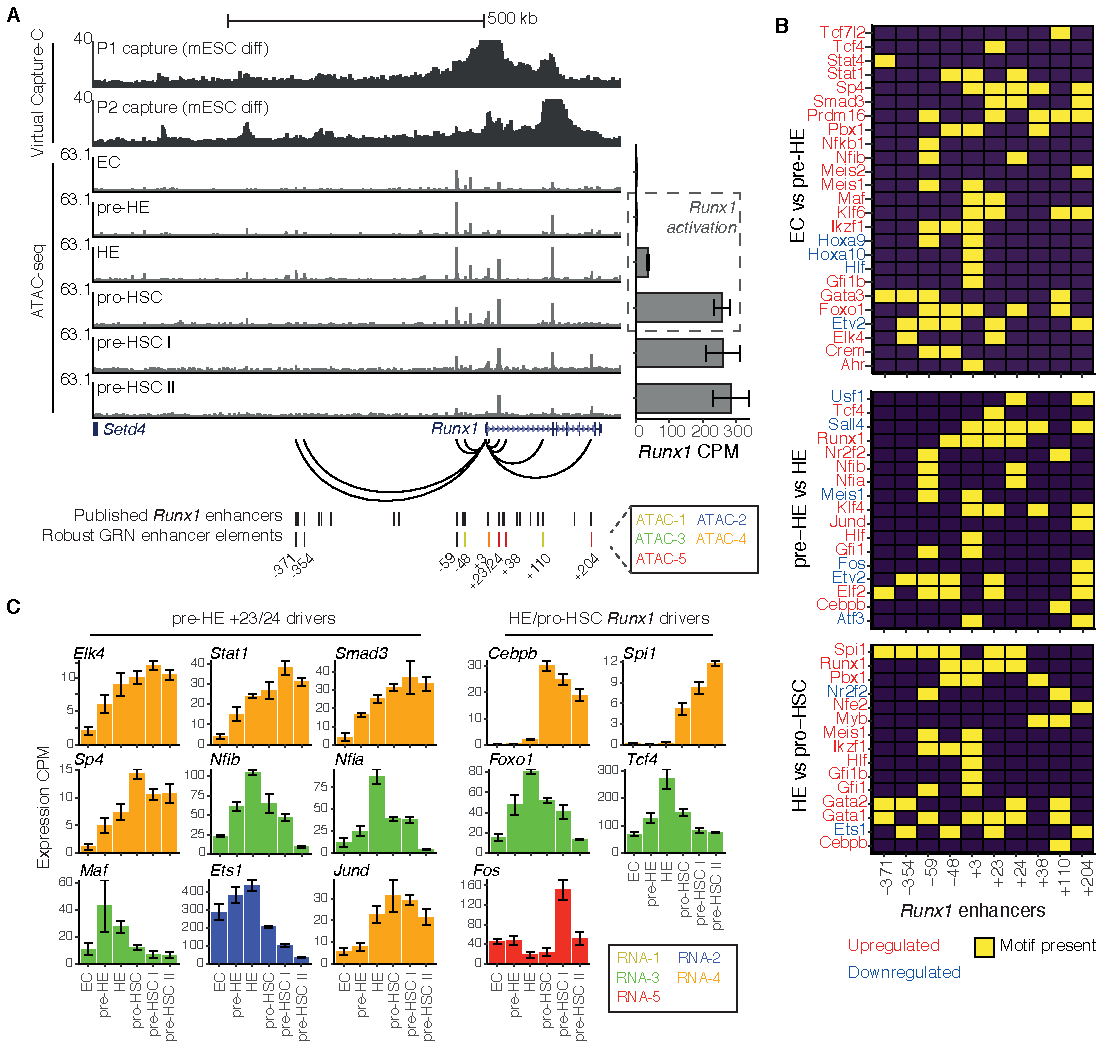
\includegraphics[width=\textwidth,height=\textheight,keepaspectratio]{figures/chapter3/ch3_runx1-regulation.png}
    \caption[{Chromatin accessibility profiles and predicted enhancers across the \textit{Runx1} locus.}]
    {\textbf{Chromatin accessibility profiles and predicted enhancers across the \textit{Runx1} locus.} 
    ATAC-seq and "virtual" capture-C tracks over the \textit{Runx1} locus and upstream gene desert. Virtual capture-C tracks were taken from tiled-C data performed on mESC differentiated derived CD41\upos{} HPCs, using the P1 and P2 promoters as anchor points \citep{owens_dynamic_2022}, to show the frequency of physical interactions between promoters and surrounding DNA. For ATAC-seq tracks, replicates were combined into a single track for visualisation. GRN predicted enhancers and published enhancers \citep{owens_dynamic_2022, marsman_dna_2017, ortt_chromatin_2008, fitch_gata3_2020, cauchy_chronic_2015, cheng_runx1_2018, harland_t-box_2021, ng_runx1_2010, bee_nonredundant_2010, nottingham_runx1-mediated_2007, schutte_experimentally_2016} were annotated, coloured by accessibility profiles (ATAC1-5). \textit{Runx1} expression shown on right. Error bars represent standard error of the mean; \textit{n} = 3; \textit{n} = 4 for pre-HE. 
    \textit{Tiled capture-C data was generated and analysed by D. Owens \citep{owens_dynamic_2022}.}
    }
    \label{fig:ch3_runx1-regulation}
\end{figure}

To predict potential regulators of \textit{Runx1}, it is necessary to first establish the cis-regulatory landscape of the \textit{Runx1} locus that may drive regulation. To accomplish this, I assembled a detailed map of in vivo chromatin accessibility over the \textit{Runx1} locus based on ATAC-seq data (Fig. \ref{fig:ch3_runx1-regulation}). The EHT GRN detects several enhancers correlating with \textit{Runx1} expression, with the strongest being +23 (\textit{R} > 0.9). These include previously published enhancers with -371, -354, -59, -48, +3, +23, +24, +110, and +204 regulatory elements (as summarised in \cite{owens_dynamic_2022}), and the +38 element which has not previously been published. The +24 element is a second peak of accessibility adjacent to the +23 enhancer, that boosts +23 activity (de Bruijn lab, unpublished). 

Of these predicted regulatory elements, -59, -48, and +23/+24 are accessible in ECs (though +23 low signal prior to HE could be due to presence of the +23GFP transgene). Low level -371 and -354 accessibility is initiated in pre-HE and increased in HE, then closed from pro-HSCs onwards (Fig. \ref{fig:ch3_runx1-regulation}). From pre-HE to HE, the +3, +23 and +24 enhancers increased accessibility. +23 and +24 remain open throughout EHT, and +3 remains accessible until closing in pre-HSC II. The -54 and -48 enhancers decreased in accessibility as EHT progressed from pro-HSCs onwards, suggesting they are silencers of the locus, or that they are only involved in initial \textit{Runx1} induction. The +38 enhancer is weakly accessible in pre-HSC populations. The +204 element is weakly accessible in pre-HE and HE, closed in pro-HSC, but strongly accessible in pre-HSC populations. Additionally, the +110 enhancer has weak activity specifically in the pro-HSC population. This increased accessibility of +110, and absence of +204 accessibility, in the pro-HSC population is likely to reflect the presence of CD43+ HPCs, as discussed in section \ref{ch3:profiling} (de Bruijn lab, unpublished). 

To evidence that these GRN predicted elements regulate \textit{Runx1}, I took tiled capture-C analysis previously performed on mESC haematopoietic differentiation populations (Flk1\upos{} mesoderm and CD41\upos{} HPCs) in the de Bruijn lab (D. Owens, \cite{owens_dynamic_2022}). These predicted regulatory elements displayed physical interaction with either the P1 or P2 promoters, though -371 and -354 showed low interaction frequency (Fig. \ref{fig:ch3_runx1-regulation}). Analysis from \cite{owens_dynamic_2022} showed -59, -48, +3, +23, and +110 enhancers to increase in P1 and P2 interactions when mESCs are differentiated from mesoderm to HPCs. Together, these analyses and observations construct a comprehensive map of \textit{Runx1} regulatory enhancers and silencers that drive \textit{Runx1} expression.

\subsection{\label{ch3:runx1-motifs}Predicted regulators of \textit{Runx1} expression}

To predict potential TFs driving \textit{Runx1} expression I aimed to explore TF binding motifs across the cis-regulatory landscape. There are three cell population transitions of particular relevance to \textit{Runx1} regulation: the EC to pre-HE transition marked by +23GFP expression \citep{swiers_early_2013}, the pre-HE to HE transition marked by initiation of endogenous \textit{Runx1} expression, and the HE to pro-HSC transition where \textit{Runx1} expression is upregulated (Fig. \ref{fig:ch3_runx1-regulation}). I interrogated potential drivers of \textit{Runx1} transcription by exploring TF binding motifs present at the enhancers of E-P interactions (Fig. \ref{fig:ch3_runx1-motifs}A-B, see methods section \ref{ch2:motifs}, p.\pageref{ch2:motifs}). Only high confidence TF motif PWMs from the HOCOMOCO motif database were used, to improve confidence of predicted regulatory interactions (core HOCOMOCO, \cite{kulakovskiy_hocomoco_2018}). Motifs were stratified by pairwise differential analyses between populations to predict transition-specific drivers. 

\begin{figure}[!t]
    \centering
    \includegraphics[width=\textwidth,height=\textheight,keepaspectratio]{figures/chapter3/ch3_runx1-motifs.png}
    \caption[{Predicted upstream regulation of \textit{RUNX1}.}]
    {\textbf{Predicted upstream regulation of \textit{RUNX1}.} 
    \textbf{(A)} Heatmap of TF binding motif presence ($\geq$ 1 motifs) at \textit{Runx1} enhancers. Motifs match TFs differentially expressed over the relevant pairwise comparisons, as indicated. Row labels refer to TFs associated with a detected motif, and coloured according to up- or downregulation over the transition. Columns refer to the individual \textit{Runx1} enhancers.
    \textbf{(B)} Gene expression (CPM) for predicted \textit{Runx1} enhancer regulators. Error bars represent standard error of the mean; \textit{n} = 3; \textit{n} = 4 for pre-HE. 
    }
    \label{fig:ch3_runx1-motifs}
\end{figure}

To characterise the factors that may establish the pre-HE state in E8.5 embryos, I first probed TFs upregulated from EC to pre-HE, with motifs in +23/24 enhancers. These include TFs associated with different motif families, such as ETS (Elk4), FOX (Foxo1), zinc fingers (Klf6, Prdm16 and Sp4), Maf-related bZIP (Maf), NFI (Nfib), SMAD (Smad3), STAT (Stat1) and basic Helic-Loop-Helic (bHLH) E2A (Tcf4) (Fig. \ref{fig:ch3_runx1-motifs}A). Among these differentially expressed TFs, \textit{Maf} expression is most specific to pre-HE (Fig. \ref{fig:ch3_runx1-motifs}B). While several of these TFs are reported targets of Runx1 \citep{wang_intersection_2011, zaidi_integration_2002}, their expression precedes \textit{Runx1} and coincides with 23GFP activity, suggesting an additional upstream regulatory role. Elements open in pre-HE, other than +23/24, include -371, -354, and +204 at low levels of accessibility, as well as -59 and -48 at high levels of accessibility (Fig. \ref{fig:ch3_runx1-regulation}). There are a number of TFs upregulated from EC to pre-HE, with predicted motifs in these enhancers. These include motif families such as GATA (Gata3), STAT (Stat4), Rel homology domain (RHD) NF-$\kappa$B (Nfkb1), three amino acid loop extension (TALE) homeobox MEIS (Meis1, Meis2) and PBX (Pbx1), Ikaros zinc finger (Ikzf1), and Creb-related bZIP (Crem). GATA motifs are found in -371, -354, and -59 elements, coinciding with \textit{Gata3} upregulation. Gata3 has recently been reported as essential in aortic endothelium for EHT progression and promotes \textit{Runx1} activity \citep{zaidan_endothelial-specific_2022}, and therefore may be important for the pre-HE population. 

Initiation of endogenous \textit{Runx1} transcription (pre-HE to HE) and \textit{Runx1} upregulation (HE to pro-HSC) are dynamic stages likely induced by key TFs. NFI motifs (Nfia and Nfib) underlie the -59 and +24 enhancers, and \textit{Nfia} and \textit{Nfib} genes are most expressed in HE (Fig. \ref{fig:ch3_runx1-motifs}A-B). Nfib was confirmed to bind to the +24 enhancer (but not the -59 element) using published ChIP-seq data in mammary cells (Appendix \ref{fig:app_runx1-upstream-chip}, \cite{shin_hierarchy_2016}). CEBP motifs were unique to the +110 enhancer, and the \textit{Cebpb} gene upregulated in both transitions. Cebpb binding to the +110 enhancer was validated using published ChIP-seq in pre-B cells (Appendix \ref{fig:app_runx1-upstream-chip}, \cite{van_oevelen_cebp_2015}). Similarly, we find AP-1 motifs (Fos and JunD) motifs underlying the +204 enhancer, and the \textit{Fos} gene is upregulated in the pre-HE to HE transition. Further, the binding of Fos and JunD to the +204 enhancer was confirmed in macrophages and T-cells using published ChIP-seq data (Appendix \ref{fig:app_runx1-upstream-chip}, \cite{roychoudhuri_bach2_2016, eichenfield_tissue_2016}). These observations suggest Cebpb, Fos and Jund as unique regulators of the +110 and +204 enhancers, respectively. \textit{Cebpb} upregulation occurs from HE to pro-HSC, while \textit{Jund} is upregulated from pre-HE to HE, potentially placing Cebpb and Jund as transition-specific drivers. Additionally, Nfia and Nfib are potential novel regulators of the +24 enhancer. It is important to acknowledge that motif analyses based on PWMs are inherently predictive, and while broadly accurate genome wide, may not correctly identify motifs at individual loci. Nevertheless, these analyses provide an interesting preliminary characterisation of potential novel regulators of \textit{Runx1} enhancers.

%Ets1 motifs are also found in the +3, -48, and -354 enhancers, with ChIP-seq evidence in MEL cells \citep{yue_comparative_2014}. 

\subsection{\label{ch3:runx1-targets}Predicted targets of Runx1}

%While endogenous \textit{Runx1} is not expressed in pre-HE, the 23GFP transgene is, indicating that TF signals promoting HE identity are received. Within the EC to pre-HE differential TF subnetwork there is low-level activation of late haematopoietic genes (RNA4, Fig. \ref{fig:ch3_pairwise}A). Activation of the transient module (RNA3), including multiple Notch pathway TFs, Nfib, and Gata3, occurs in pre-HE, preceding \textit{Runx1} expression. This transient regulation increases in pre-HE to HE, with the addition of TFs such as Sox17, which is known to characterise HE \citep{clarke_expression_2013}, and commitment to the haematopoietic lineage with Runx1, Gfi1 and Cebpb. The HE to pro-HSC subnetwork is dominated by committed haematopoietic TFs, such as Myb, Gfi1b and Ikzf1 (Fig. \ref{fig:ch3_pairwise}A). 

\begin{figure}[!t]
    \centering
    \includegraphics[width=\textwidth,height=\textheight,keepaspectratio]{figures/chapter3/ch3_pairwise.png}
    \caption[{Transition specific TF sub-networks highlight predicted and Runx1 targets.}]
    {\textbf{Transition specific TF sub-networks highlight predicted Runx1 targets.} 
    \textbf{(A)} Sub-networks of EHT GRN (Fig. \ref{fig:ch3_eht-grn}C) illustrating up and downregulated TFs between pre-HE and HE (left) or HE and pro-HSC (right). Nodes are coloured based on expression modules (RNA1-5). Top sub-networks show all differential TFs, and bottom sub-networks show TFs predicted to be regulated by Runx1.
    }
    \label{fig:ch3_pairwise}
\end{figure}

The GRN model predicts Runx1 to regulate many gene targets. An important consideration of these predictions is that RUNX motifs were detected based on a PWM that extends beyond the core consensus motif \citep{kulakovskiy_hocomoco_2018}, and as such likely overestimates predicted Runx1 targets. Despite this caveat, this model offers an exploration of potential Runx1 TF targets. To find key Runx1 targets that may drive EHT, I explored TFs that are differentially expressed between cell type transitions. Direct Runx1 targets are likely to be among those that change in expression just after \textit{Runx1} is upregulated, which is best represented by the pre-HE to HE, and HE to pro-HSC transitions. The GRN model in these transitions detects known Runx1 targets, such as \textit{Spi1} (PU.1) \citep{huang_pu1_2008}, \textit{Gfi1} \citep{wilson_gfi1_2010}, \textit{Nfe2} \citep{wang_aml1_2010} and \textit{Ikzf1} \citep{iacovino_hoxa3_2011} (Fig. \ref{fig:ch3_pairwise}). \textit{Zeb2} is an interesting target that was recently found to be a direct target of Runx1 in a murine kidney cell line, where expression of \textit{Zeb2} in \textit{Runx1} knockout models was sufficient to partially restore the transcriptional phenotype of Runx1 \citep{hass_runx1_2021}. Zeb2 is a known EMT regulator that represses cell-cell junction genes and promotes haematopoietic differentiation \citep{vandewalle_sip1zeb2_2005, li_emt_2017}, and as such may drive the morphological changes that underlie EHT. \textit{Cebpb} is also predicted to be a Runx1 target, and has been previously shown to regulate several key haematopoietic TFs, such as \textit{Gata2} \citep{goode_dynamic_2016}. As shown in Fig. \ref{fig:ch3_runx1-motifs}, Cebpb may regulate the +110 \textit{Runx1} enhancer, resulting in a possible positive feedback loop.

To find key Runx1 targets that may drive EHT, I examined predicted targets that are highly central, as analysed in Fig. \ref{fig:ch3_centrality}A. \textit{Etv2} is a highly central TF in the RNA1 module, with biased expression towards endothelium, that is predicted to be regulated by Runx1 (Fig. \ref{fig:ch3_pairwise}). Interestingly, \textit{Etv2} is expressed in mesoderm and drives both endothelial and haematopoietic programs \citep{liu_induction_2015, menegatti_transcriptional_2019}, and acts as a precursor of HE and EC fate. \textit{Runx1} expression defines the haematopoietic fate of Etv2+ endothelial progenitors \citep{eliades_hemogenic_2016}, and from this analysis may directly repress \textit{Etv2}, in line with the known role of Runx1 to repress the endothelial program \citep{lancrin_gfi1_2012}. Ikzf1 is a prominent central TF in the RNA5 module (late haematopoietic expression) (Fig. \ref{fig:ch3_centrality}A), and is a GRN predicted, and known target of \textit{Runx1} (Fig. \ref{fig:ch3_pairwise}), as has been previously reported in mESC derived EBs \citep{iacovino_hoxa3_2011}. Ikzf1 is expressed in multiple haematopoietic lineages, and is critical for B cell development \citep{nichogiannopoulou_defects_1999,georgopoulos_making_2017,marke_many_2018}. 

This analysis has predicted several known, and novel targets of Runx1. The role of several of these targets, such as Ikzf1, Zeb2, and Cebpb, is not fully understood. It remains a question as to whether Runx1 regulation is important for their normal function and contribution to EHT.

\section{\label{ch3:co-interaction}Runx1 cooperates with TFs to drive EHT processes}

The analysis of the EHT GRN thus far has identified regulatory modules underlying key transitions (section \ref{ch3:profiling}, Fig. \ref{fig:ch3_clusters}), the candidate drivers of each module (section \ref{ch3:centrality}, Fig. \ref{fig:ch3_centrality}), as well as the regulatory context of Runx1 (section \ref{ch3:runx1-context}, Fig. \ref{fig:ch3_runx1-regulation}, Fig. \ref{fig:ch3_runx1-motifs}, and Fig. \ref{fig:ch3_pairwise}). An important consideration in gene regulation is that TFs often do not act independently. While some TFs may act as pioneer factors in specific contexts \citep{zaret_pioneer_2016, zaret_pioneer_2020} and so can function independent of other factors, it is also common for TFs to act in complex with other proteins. The bZIP class of TFs is a classic example of dimerising proteins that modulate TF behaviour \citep{rodriguez-martinez_combinatorial_2017, miller_importance_2009}. Runx1 is also known to cooperate with multiple other TFs \citep{wang_intersection_2011, zaidi_integration_2002, hu_runx1_2011, kim_mutual_1999, goetz_auto-inhibition_2000}, and the expression of \textit{Runx1} leads to genome-wide modulation of Fli1 DNA binding affinities \citep{lichtinger_runx1_2012}. TF cooperation is challenging to explore on a genome-wide scope, but a study of how TFs may cooperate in EHT may offer greater insight into the regulation of EHT. 

\begin{figure}[!t]
    \centering
    \includegraphics[width=\textwidth,height=\textheight,keepaspectratio]{figures/chapter3/ch3_TF-cointeraction.png}
    \caption[{TFs cooperate in clusters to drive different EHT processes.}]
    {\textbf{TFs cooperate in clusters to drive different EHT processes.} 
    \textbf{(A)} Hierarchical clustered heatmap of odds ratios resulting from Fishers Exact tests comparing the overlap of TF-targets (enhancers) between pairs of TFs. Benjamini and Hochberg correction of P values was performed, and TFs not significant for any interaction were excluded. Clusters describe sets of TFs that commonly act at the same loci, suggesting cooperative regulation. 
    \textbf{(B)} GO biological process enrichment for clusters CoInt 1-4, as in A. Only significant data points shown (P $\leq$ 0.05). Note that no terms were significantly enriched for CoInt-5 .
    \textbf{(C)} Frequency of TFs in each CoInt cluster, as in A, stratified by RNA expression modules (RNA1-5). 
    \textbf{(D)} Stratification of degree (left) and betweenness centrality (right) of the EHT GRN, stratified by CoInt clusters. Only TFs found to significantly co-interact with Runx1 are shown (FDR < 0.05). 
    }
    \label{fig:ch3_TF-cointeraction}
\end{figure}

Here I aimed to apply the GRN model to predict potential cases of TF cooperativity. To predict TF co-interaction in the EHT GRN, I designed an approach to find TF pairs that are predicted to commonly regulate the same enhancer or promoter element. Note that in this thesis I am using "cooperativity" to refer to TFs that function synergistically, and "co-interaction" to refer to TFs predicted to regulate the same sites, as without additional experiments, synergy cannot be proven using the GRN model alone. I performed Fisher's exact tests for all possible TF pairs, in which a positive odds ratio describes TFs that co-interact more frequently than if interactions were random. Odds ratio scores were then grouped into five co-interaction clusters (CoInt 1-5, Fig. \ref{fig:ch3_TF-cointeraction}A). These clusters represent TFs that are predicted to co-interact at the same loci, and by GO analyses each cluster is enriched for different processes (Fig. \ref{fig:ch3_TF-cointeraction}B). Runx1 is in CoInt-1, which is enriched for multiple haematopoietic lineage differentiation processes, in line with driving a haematopoietic program (Fig. \ref{fig:ch3_TF-cointeraction}B). CoInt-2 is related to the stress response, and CoInt-3 involves cell cycle genes and responses to external factors. Interestingly, CoInt-4 is associated with blood vessel morphogenesis and EMT, suggesting a role in modulating aortic endothelium and driving morphological changes.

TFs in CoInt1-3 are enriched in the GRN module RNA4, so are activated in HE or pro-HSCs (Fig. \ref{fig:ch3_TF-cointeraction}C). CoInt-4/5 TFs are instead enriched in the transient expression module (RNA3), and likely represent a cooperative program that drives the effects of the transient module. This is emphasised by CoInt-4 driving EMT processes, in line with RNA3 association with EMT and actin cytoskeletal organisation. Interestingly, when exploring \textit{Runx1} expression correlation with predicted Runx1 targets across GRN modules, \textit{Runx1} is found positively correlated with RNA4-5, but is anti-correlated with RNA-3 (Appendix \ref{fig:app_runx1-cor}). This suggests that Runx1 activity represses transiently expressed genes. Runx1 co-interactors are primarily found in CoInt-1 and CoInt-2 (RNA4 enriched), but not CoInt-4 or CoInt-5 (RNA3 enriched) (Fig. \ref{fig:ch3_TF-cointeraction}C), suggesting that while Runx1 may regulate the transient program (RNA3), it does not cooperate with transient TFs. Runx1 co-interacts with multiple highly central TFs (Fig. \ref{fig:ch3_TF-cointeraction}D), including factors known to cooperate with Runx1 such as Fli1 \citep{lichtinger_runx1_2012}, PU.1 \citep{hu_runx1_2011}, and Ets1 \citep{kim_mutual_1999, goetz_auto-inhibition_2000}. Several TFs that co-interact with Runx1 also display high betweenness centrality, such as Etv6, Ets1, Ikzf1, and Sp4 (Fig. \ref{fig:ch3_TF-cointeraction}D, Fig. \ref{fig:ch1_stress-example}, p.\pageref{fig:ch1_stress-example}). Several of these are predicted targets of Runx1, including Ets1 and Ikzf1. These high betweenness centrality nodes may be critical for GRN pathways, and may cooperate with Runx1. 

\begin{figure}[!t]
    \centering
    \includegraphics[width=\textwidth,height=\textheight,keepaspectratio]{figures/chapter3/ch3_sc-rna.png}
    \caption[{Gene expression correlation between CoInt-1 TFs in scRNA-seq data.}]
    {\textbf{Gene expression correlation between CoInt-1 TFs in scRNA-seq data.} 
    \textbf{(A, B)} UMAP analysis of mouse EHT scRNA-seq from \cite{zhu_developmental_2020} (A), and Force directed graph (ForceAtlas2, FA2) of human EHT scRNA-seq from \cite{zeng_tracing_2019} (B). Sort populations labelled on left plots. Right plots show Slingshot pseudotime scores. Arrows represent direction of cell differentiation.
    \textbf{(C, D)} Correlation heatmaps of scRNA-seq expression from \cite{zhu_developmental_2020} (C) and \cite{zeng_tracing_2019} (D). See methods section \ref{ch2:pseudo}, p.\pageref{ch2:pseudo} for single cell correlation calculation. 
    \textbf{(E)} scRNA-seq expression of key Runx1 co-interacting TFs for mouse (top) and human (bottom) over pseudotime. Lines indicate smooth fitted values calculated by TradeSeq analysis. 
    \textit{Raw scRNA-seq data from \cite{zhu_developmental_2020} and \cite{zeng_tracing_2019}, reanalysed by me.} 
    }
    \label{fig:ch3_sc-rna}
\end{figure}

This analysis successfully identifies TFs that commonly co-interact co-interact at the same loci, and specifically explores TFs that co-interact with Runx1. However, it does not provide evidence for synergistic cooperativity. Further, the GRN model is based on defined populations from bulk RNA-seq and ATAC-seq, and the relationship between these TFs may differ on a single cell level. To address this, I reanalysed published scRNA-seq EHT datasets in human and mouse \citep{zeng_tracing_2019, zhu_developmental_2020}. To compare gene expression patterns to \textit{Runx1} transcription, I performed pseudotime analysis and correlated gene expression using expression values smoothed along the pseudotime axis (Fig. \ref{fig:ch3_sc-rna}A-B, methods section \ref{ch2:pseudo}, p.\pageref{ch2:pseudo}). This revealed CoInt-1 TFs can be either correlated or anti-correlated with \textit{Runx1} expression (Fig. \ref{fig:ch3_sc-rna}C-E). \textit{Ets1}, \textit{Zeb1} and \textit{Snai1} were consistently anti-correlated with \textit{Runx1}, which may suggest that these factors cooperate with Runx1 in a very specific window before downregulation. Other TFs were positively correlated with \textit{Runx1} expression, with \textit{Etv6}, \textit{Spi1}, \textit{Myb}, \textit{Elf1}, and \textit{Ikzf1} showing the highest correlation. This positive correlation suggests these factors may synergistically cooperate, though further study is required. Overall, this analysis predicts significant TF co-interaction throughout EHT, and this cooperative logic may drive specific EHT processes.

\section{Potential Runx1 driven FFLs in EHT}

This framework to interrogate predicted TF cooperation allowed us to begin exploring how combinatorial regulatory logic may drive different regulatory processes. A common circuit in which TF cooperation occurs is through a FFL, where one TF regulates another TF, and both TFs cooperate to drive regulation of a downstream gene (section \ref{ch1:grn-motifs}, p.\pageref{ch1:grn-motifs}). FFLs are also highly enriched in biological networks \citep{milo_network_2002, mangan_structure_2003}, and are thought to mediate particular gene expression dynamics such as enacting sign-senstive delay in response to signals \citep{mangan_coherent_2003, kalir_coherent_2005}, and acting as pulse generators \citep{mangan_structure_2003, basu_spatiotemporal_2004}. 

\begin{figure}[!t]
    \centering
    \includegraphics[width=\textwidth,height=\textheight,keepaspectratio]{figures/chapter3/ch3_runx1-TF-motifs.png}
    \caption[{Motif enrichment of Runx1 co-interacting TFs across ATAC-seq accessibility modules.}]
    {\textbf{Motif enrichment of Runx1 co-interacting TFs across ATAC-seq accessibility modules.} 
    \textbf{(A)} Heatmap of TF DNA binding motif enrichment scores (-log\textsubscript{10} E-value) (MEME-AME, methods section \ref{ch2:motifs}, p.\pageref{ch2:motifs}) within ATAC-seq elements found in modules ATAC1-5. Rows indicate peak sets from ATAC1-5 modules, columns indicate motif enrichment. Column labels refer to TFs (as in CoInt-1 and CoInt-2 co-interactions clusters) for which a motif PWM is associated, and used for enrichment analysis. TFs in CoInt-1 and CoInt-2 that co-interact with Runx1 shown. TF labels are coloured red if they are GRN predicted targets of Runx1, or green if they are predicted targets of Runx1 and are differentially expressed in either the pre-HE to HE, or HE to pro-HSC transitions (see Fig. \ref{fig:ch3_pairwise}). 
    \textbf{(B)} Relationship between motif enrichment scores at ATAC-seq modules (ATAC1-5), and proportion of elements in each module containing motif. Note the motif for Hes1 was sourced from the full HOCOMOCO TF motif database (see section \ref{ch2:motifs}, p.\pageref{ch2:motifs} for database details). Nodes highlighted in red include the Hes1 motif, and TF motifs associated with predicted Runx1 targets, differentially expressed the pre-HE to HE or HE to pro-HSC transitions.
    }
    \label{fig:ch3_runx1-TF-motifs}
\end{figure}

Several TFs within CoInt-1 and CoInt-2 were found to frequently co-interact with Runx1, such as the high betweenness centrality TFs Etv6, Ets1, Sp4, and Ikzf1 (Fig. \ref{fig:ch3_TF-cointeraction}C-D). Additionally, a number of these co-interacting TFs were also found to be targets of Runx1, and in particular were differentially expressed subsequent to the onset of \textit{Runx1} expression. These include Ets1, Ikzf1, Meis1, Nfe2, PU.1, Mef2c, Gfi1, Pbx1, and Cebpb (Fig. \ref{fig:ch3_runx1-TF-motifs}A, Fig. \ref{fig:ch3_pairwise}, Fig. \ref{fig:ch3_TF-cointeraction}), suggesting that Runx1 has the capacity to form cooperative FFLs with these TFs. I next probed what processes these co-interacting TFs may regulate. While the majority of CoInt-1 and CoInt-2 TFs are expressed in RNA4 and RNA5 modules (Fig. \ref{fig:ch3_TF-cointeraction}C), they may not necessarily interact with ATAC4 and ATAC5 accessible elements. To determine what ATAC-seq modules CoInt-1 and CoInt-2 TFs are most likely to regulate, I performed TF binding motif enrichment analysis across ATAC1-5 elements (Fig. \ref{fig:ch3_runx1-TF-motifs}A). For example, RUNX motifs are highly enriched in ATAC5 over other modules, suggesting Runx1 binds to and regulates pre-HSC-active genes. This analysis does not preclude Runx1 from regulating targets in other modules, and in-fact many of the TFs predicted to co-interact with Runx1 are instead associated with endothelial and transient accessible sites (ATAC2 and ATAC3). Runx1 may therefore cooperate with TFs across different ATAC-seq accessibility modules, in possible FFL configurations. 

ETS motif TFs (Ets1, PU.1) are enriched in ATAC-seq modules ATAC2, ATAC3 and ATAC5, with some specificity differentiating PU.1 and Ets1 HOCOMOCO PWMs resulting in higher enrichment for the PU.1 PWM in ATAC5 (Fig. \ref{fig:ch3_runx1-TF-motifs}A-B). Motifs for Meis1 and Nfe2 are enriched in ATAC2 peaks, suggesting that they interact with the endothelial program (Fig. \ref{fig:ch3_runx1-TF-motifs}A-B). Meis1 has been reported to promote EC development in zebrafish \citep{minehata_meis1_2008}, and \textit{Meis1} knockout studies result in abnormal vasculature \citep{hisa_hematopoietic_2004}. Pbx1 motifs are enriched in both ATAC3 and ATAC4 elements (Fig. \ref{fig:ch3_runx1-TF-motifs}A-B), and Pbx1 is known to mediate HSC quiescence, possibly through activation of Tgf-$\beta$ related genes \citep{ficara_pbx1_2008}, and as such may regulate Tgf-$\beta$ activity in IAC populations. Motifs for Ikzf1, Mef2c and Gfi1 are biased towards ATAC3 (Fig. \ref{fig:ch3_runx1-TF-motifs}A-B), suggesting these factors regulate the transiently accessible module. Mef2c is known for its roles in megakaryopoiesis and B-cell development \citep{gekas_mef2c_2009}, and Ikzf1 is a TF critically required for B-cell development \citep{nichogiannopoulou_defects_1999}, though their role in EHT is unclear.

\begin{figure}[!t]
    \centering
    \includegraphics[width=\textwidth,height=\textheight,keepaspectratio]{figures/chapter3/ch3_runx1-ikzf1-notch.png}
    \caption[{Runx1 and Ikzf1 cooperate to repress the Notch pathway through a Runx1:Ikzf1:\textit{Hes1} FFL.}]
    {\textbf{Runx1 and Ikzf1 cooperate to repress the Notch pathway through a Runx1:Ikzf1:\textit{Hes1} FFL.} 
    \textbf{(A)} Relationship between enrichment of TF motifs at ATAC3 elements, and the number of GRN predicted TF targets in the Notch pathway (GO:0007219). 
    \textbf{(B)} TF interaction matrix showing predicted regulation of TFs at Notch pathway targets. TF regulators are shown as columns, and predicted Notch pathway targets as rows. 
    \textbf{(C)} Correlation heatmaps from scRNA-seq EHT data. 
    \textbf{(D)} Circuit illustrating predicted regulation of Notch genes by Runx1 (light grey lines) and Ikzf1 (dark grey lines). 
    \textbf{(E)} Gene expression (CPM) for \textit{Runx1}, \textit{Ikzf1}, and select Notch genes. Error bars represent standard error of the mean; \textit{n} = 3; \textit{n} = 4 for pre-HE. 
    \textit{Raw scRNA-seq data from \cite{zhu_developmental_2020} and \cite{zeng_tracing_2019}, reanalysed by me.} 
    }
    \label{fig:ch3_runx1-ikzf1-notch}
\end{figure}

\subsection{\label{ch3:notch}A Runx1 and Ikzf1 driven FFL regulates Notch pathway genes}

An interesting aspect of Runx1 activity in the EHT GRN model is that Runx1 targets in the RNA3 expression module are anti-correlated with \textit{Runx1} expression (Appendix \ref{fig:app_runx1-cor}), suggesting that Runx1 represses genes in the transient network. I next explored the capacity for Runx1, in cooperation with other TFs, to repress transiently expressed genes. In section \ref{ch3:profiling}, I found the transient expression and accessibility modules (RNA3 and ATAC3) to be enriched for Notch signalling by GO analysis (Fig. \ref{fig:ch3_clusters}C-D). Interestingly, motifs for the Notch target gene, \textit{Hes1}, are also highly enriched at transient elements (ATAC3, Fig. \ref{fig:ch3_runx1-TF-motifs}B). This suggests that Notch signalling is a prominent regulator of the transient EHT network. I screened all TFs enriched in ATAC3 for possible regulation of the Notch pathway, by quantifying the number of GRN predicted targets at Notch signalling related genes (GO:0007219) (Fig. \ref{fig:ch3_runx1-ikzf1-notch}A). The TFs that were found to most frequently target the Notch pathway within the GRN model were Ikzf1, PU.1 and Ets1. Previous study identified Ikzf1 as a repressor of Notch signalling in T-cell development \citep{kleinmann_ikaros_2008}, and this analysis suggests that this activity is present in EHT as well. Ikzf1 is of particular interest, as it is predicted to be regulated by Runx1 (section \ref{ch3:runx1-targets}, Fig. \ref{fig:ch3_pairwise}), is found to co-interact with Runx1 (section \ref{ch3:co-interaction}, Fig. \ref{fig:ch3_TF-cointeraction}), and is a highly central TF within the RNA5 gene expression module (section \ref{ch3:centrality}, Fig. \ref{fig:ch3_centrality}), suggesting it is an active driver of late-EHT populations. IKZF motifs are significantly enriched at all ATAC-seq modules, but most enriched at transiently accessible (ATAC3) sites (Fig. \ref{fig:ch3_runx1-TF-motifs}B). As Ikzf1 can deactivate targets through recruitment of HDAC \citep{marke_many_2018}, and its motif is highly enriched at transiently accessible (ATAC3) sites, this positions it as a potential repressor of the transient EHT network. More specifically, it may repress Notch pathway genes, which is a known behaviour of Ikzf1 in T-cell development \citep{kleinmann_ikaros_2008}, but is an as yet unexplored interaction in EHT. 

As \textit{Ikzf1} is a predicted target of Runx1, and Ikzf1 co-interacts with Runx1, it is possible that these factors cooperate at Notch genes in a FFL circuit. While Ikzf1 is predicted to regulate many Notch genes, Runx1 is predicted to regulate relatively few, such as \textit{Notch1} and \textit{Hes1} (Fig. \ref{fig:ch3_runx1-ikzf1-notch}B). Ikzf1 also regulates these loci, and additionally targets \textit{Hey1}, \textit{Hey2}, \textit{Jag1} and \textit{Dll4}. I used the mouse and human scRNA-seq EHT data from \cite{zhu_developmental_2020} and \cite{zeng_tracing_2019}, respectively, to compare expression profiles (Fig. \ref{fig:ch3_runx1-ikzf1-notch}C). \textit{Runx1} expression was strongly anti-correlated with \textit{Hes1} and \textit{Notch1}, but not \textit{Hey1} or \textit{Hey2} (Fig. \ref{fig:ch3_runx1-ikzf1-notch}C), in line with its predicted regulation. \textit{Ikzf1} was instead anti-correlated with each of its predicted targets. Together, this suggests a key role for Ikzf1 in repressing Notch signalling, and may cooperate with Runx1 at a subset of Notch pathway genes. GRN predicted interactions downstream of Runx1 and Ikzf1 suggest a FFL circuit, where Runx1 activates \textit{Ikzf1}, and both TFs cooperate to repress \textit{Notch1} and \textit{Hes1} (Fig. \ref{fig:ch3_runx1-ikzf1-notch}D). Additionally, a TF cascade is predicted where Ikzf1 regulates several Notch genes independently of Runx1. Based on expression data, Runx1 does not appear to be sufficient to fully repress \textit{Notch1} or \textit{Hes1} alone, and full inactivation of these genes does not occur until \textit{Ikzf1} is upregulated in pre-HSC I and pre-HSC II populations (Fig. \ref{fig:ch3_runx1-ikzf1-notch}E). This is in line with the hypothesis that Runx1 and Ikzf1 can cooperate with each other, and may synergise to maximise repression of the Notch pathway.

\begin{figure}[!b]
    \centering
    \includegraphics[width=0.9\textwidth,height=\textheight,keepaspectratio]{figures/chapter3/ch3_runx1-ikzf1.png}
    \caption[{Validation of Runx1:\textit{Ikzf1} interaction.}]
    {\textbf{Validation of Runx1:\textit{Ikzf1} interaction.} 
    \textbf{(A)} Capture-C tracks over the \textit{Ikzf1} locus (top), using the \textit{Ikzf1} promoter as the capture point (dashed line). Reads normalised as 416B signal (active \textit{Runx1}) over mESC signal (inactive \textit{Runx1}). Runx1 and H3K27ac ChIP-seq from 416B cells (bottom). GRN enhancer elements annotated. 
    \textbf{(B)} qRT-PCR assaying \textit{Runx1} and \textit{Ikzf1} expression at day 7 of differentiation of \textit{Runx1}\textsuperscript{+/+} and \textit{Runx1}\textsuperscript{-/-} mESC lines (\textit{n} = 3). Expression normalised to \textit{Atp5a1} and \textit{Gapdh}. ns: not significant, * P < 0.05 , ** P < 0.01. 
    \textit{Capture-C (A) performed and analysed by D. Owens, and qRT-PCR (B) performed by L. Greder. ChIP-seq data (A) sourced from \cite{schutte_experimentally_2016} and analysed by me.} 
    }
    \label{fig:ch3_runx1-ikzf1}
\end{figure}

To functionally validate the existence of these FFL circuits (Fig. \ref{fig:ch3_runx1-ikzf1-notch}D), it is first important to explore the Runx1 driven regulation of \textit{Ikzf1}. The EHT GRN predicted Runx1 to regulate the -28, -112, and -121 kb \textit{Ikzf1} enhancers upstream of the promoter. The -121 and -28 elements were characterised in \cite{alomairi_integration_2020}, where the -121 element was found to be a strong enhancer in CD4\upos{}CD8\upos{} T-cells. The enhancer potential, and relevance of these enhancer elements to EHT, is as yet unclear, but may act to drive Runx1 and Ikzf1 FFLs. To validate that these have enhancer features, I reanalysed published Runx1 and H3K27ac ChIP-seq data in 416B cells (CD34+ myeloid cell line) \citep{schutte_experimentally_2016}, and capture-C analysis performed by D. Owens (de Bruijn lab). These data found the -28, -112 and -121 elements were bound by Runx1 and marked by H3K27ac, and to physically interact with the \textit{Ikzf1} promoter (Fig. \ref{fig:ch3_runx1-ikzf1}A). Runx1 was functionally validated to regulate \textit{Ikzf1} by L. Greder (de Bruijn lab), who showed that \textit{Ikzf1} expression was reduced in \runxnull{} cells (Fig. \ref{fig:ch3_runx1-ikzf1}B). Further work from L. Greder (de Bruijn lab, unpublished) has functionally tested the Runx1:Ikzf1:\textit{Hes1} FFL circuit in mESC differentiation cultures (Appendix \ref{fig:app_notch-ffl-validation}). This experiment used \textit{Ikzf1\textsuperscript{-/-}} and \textit{Ikzf1\textsuperscript{+/+}} mESCs, and used a \textit{Runx1-ERt2} fusion to control Runx1 nuclear translocation. Ikzf1 and Runx1 activity is referred to here as active (Ikzf1+/Runx1+) or inactive (Ikzf1-/Runx1-). It was found that in Ikzf1-/Runx1+ conditions, Runx1 appears to promote \textit{Hes1} expression over Ikzf1-/Runx1- conditions (Appendix \ref{fig:app_notch-ffl-validation}), contrary to the GRN-predicted activity of Runx1 at this locus. In Ikzf1+/Runx1- conditions, \textit{Hes1} is instead repressed compared with Ikzf1-/Runx1- conditions, in line with the predicted repressive activity of Ikzf1. Interestingly, \textit{Hes1} is maximally repressed only in Ikzf1+/Runx1+ conditions, suggesting that both Runx1 and Ikzf1 are required for full downregulation of the gene. These analyses build evidence for a functional Runx1:Ikzf1:\textit{Hes1} FFL circuit that drives repression of \textit{Hes1}, and is a potential mechanism to drive Notch pathway suppression in pre-HSC I and pre-HSC II populations where \textit{Ikzf1} is expressed.


\section[Maf and Lef1 cooperation may drive cytoskeletal remodelling and EMT processes]{\label{ch3:maf-lef1}Maf and Lef1 cooperation may drive\\cytoskeletal remodelling and EMT processes}

The data thus far showcases the utility of the analytical strategy for predicting novel cooperative regulation driving key processes. I next aimed to explore potential TF cooperation involving factors other than Runx1. During EHT, the morphological changes and budding of HE is an important process for the formation and maturation of IACs. Among TF co-interaction clusters, TFs in CoInt-4 were transiently expressed (RNA3) and enriched for blood vessel morphogenesis and EMT (Fig. \ref{fig:ch3_TF-cointeraction}B-C), reflecting the EHT budding process. TFs in CoInt-4 also have an overall greater proportion of targets within actin cytoskeletal remodelling and EMT pathways than other co-interaction clusters (Fig. \ref{fig:ch3_maf1-lef1}A). Of these, the Maf family of TFs is predicted to regulate a high number of both actin cytoskeletal remodelling and EMT genes. Maf and Maff are bZIP TFs that share a highly similar DNA binding motif. Maf forms homodimers and contains a potent transactivating domain, while Maff lacks a transactivating domain but regulates gene targets through heterodimerising with other bZIP TFs \citep{kataoka_multiple_2007, katsuoka_small_2016}. As noted earlier, MAF motifs are found in the +3 and +23 \textit{Runx1} enhancers (Fig. \ref{fig:ch3_runx1-regulation}B), suggesting they may play a role in the activity of these enhancers.

\begin{figure}[htbp]
    \centering
    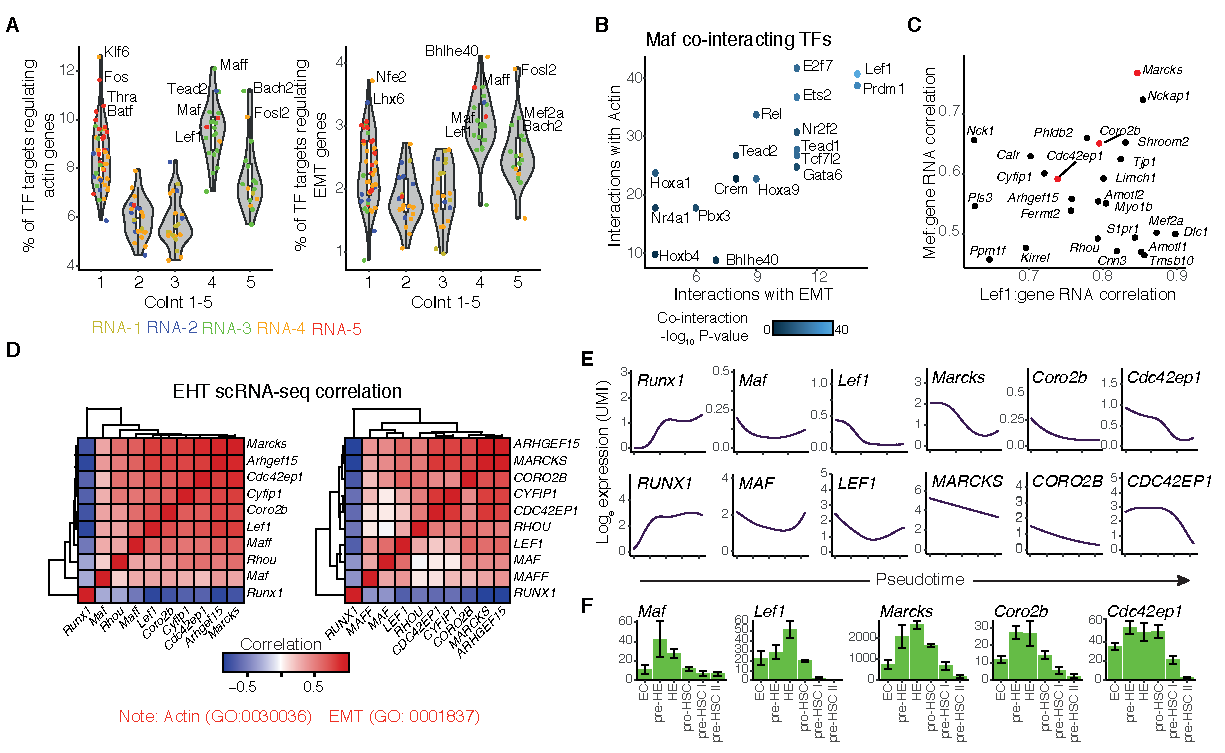
\includegraphics[width=\textwidth,height=\textheight,keepaspectratio]{figures/chapter3/ch3_maf-lef1.png}
    \caption[{The transient co-interaction module is predicted to drive cytoskeletal rearrangement through Maf:Lef1 cooperative action.}]
    {\textbf{The transient co-interaction module is predicted to drive cytoskeletal rearrangement through Maf:Lef1 cooperative action.} 
    \textbf{(A)} Proportion of TF targets that regulate actin cytoskeletal organisation (GO:0030036, left) and EMT (GO:0001837, right), across co-interaction clusters. Colour represents RNA expression modules. 
    \textbf{(B)} Frequency of TF targets regulating actin cytoskeletal organisation and EMT pathways. TFs shown significantly co-interact with Maf (FDR < 0.05). 
    \textbf{(C)} Gene expression correlation of actin cytoskeletal organisation genes, and \textit{Maf} or \textit{Lef1}. Genes of interest highlighted in red. 
    \textbf{(D)} Correlation heatmaps from scRNA-seq EHT data. 
    \textit{Legend continued on next page.}
    }
    \label{fig:ch3_maf1-lef1}
\end{figure}

There are several genes that significantly co-interact with Maf, but relatively few of these prominently interact with actin or EMT related genes (Fig. \ref{fig:ch3_maf1-lef1}B). Lef1 is a CoInt-3 TF that interacts highly with both pathways and is among the most central regulators of the transient expression module (Fig. \ref{fig:ch3_centrality}A). Of actin genes, both \textit{Maf} and \textit{Lef1} gene expression is highly correlated with \textit{Marcks} and \textit{Nckap1} expression, and moderately correlated with \textit{Cdc42ep1} (Fig. \ref{fig:ch3_maf1-lef1}C). Marcks is a membrane-bound or cytoplasmic protein that drives cytoskeletal rearrangement and migration, and has been implicated in EMT \citep{el_amri_marcks_2018, xiang_myristoylated_2019}. Cdc42ep1 (also known as Borg5) is associated with Cdc42, a key regulator of actin dynamics, and drives directional migration and angiogenesis \citep{liu_borg5_2014, farrugia_borg_2016, watson_cdc42_2016}. Nckap1 (HEM-2) is a component of the WAVE complex, which promotes activity of Arp2/3 to drive actin branching \citep{chen_structure_2010, chen_wave_2014}. To reinforce this model of Maf and Lef1 regulating actin related genes I used the EHT scRNA-seq data from \cite{zhu_developmental_2020} and \cite{zeng_tracing_2019}. Many of the actin-related genes are correlated with each other, as well as with \textit{Maf} and \textit{Lef1} expression (Fig. \ref{fig:ch3_maf1-lef1}D). Note that these scRNA-seq data consist of E9.5 and E10.5 populations, and so captures the end of EHT. Single cell pseudotime analysis shows \textit{Maf}, \textit{Lef1}, and actin genes to decrease in expression over time, in line with bulk RNA-seq expression patterns from E9.5 HE to E10.5 pre-HSC II (Fig. \ref{fig:ch3_maf1-lef1}E-F). This analysis supports a model whereby Maf1 and Lef1 cooperate to drive morphological changes, though this has yet to be experimentally validated. 
\begin{figure}[!t]
    \ContinuedFloat
    \hrule
    \vspace{5mm}
    \caption[]
    {\textit{Legend continued from previous page}. \textbf{(E)} scRNA-seq expression of \textit{Maf}, \textit{Lef1}, and key actin related genes for mouse (top) and human (bottom) over pseudotime. Lines indicate smooth fitted values calculated by TradeSeq. 
    \textbf{(F)} Gene expression (CPM) for \textit{Maf}, \textit{Lef1}, and key actin related genes in bulk RNA-seq data. Error bars represent standard error of the mean; \textit{n} = 3; \textit{n} = 4 for pre-HE. 
    \textit{Raw scRNA-seq data from \cite{zhu_developmental_2020} and \cite{zeng_tracing_2019}, reanalysed by me.} 
    }
\end{figure}
\vspace*{3in}

\clearpage
\section{Conclusions and discussion}

In this chapter, I aimed to explore potential mechanisms by which EHT regulation is driven. Through the integration of RNA-seq and ATAC-seq datasets, I have established a GRN model that predicts TF regulation that may drive activity of complex regulatory patterns associated with EHT. Using this GRN model I characterised predicted upstream regulators, and downstream targets, of Runx1. Taking advantage of these predicted interactions, I performed an analysis predicting possible TF cooperation that may drive EHT programs. One of these predicted TF cooperations was a Runx1:Ikzf1 driven FFL that represses Notch pathway genes. This FFL may contribute to deactivation of the transiently regulated EHT program, as the Hes1 motif underlies many transiently accessible enhancers (Fig. \ref{fig:ch3_runx1-TF-motifs}B).

While several studies have established GRN models of EHT \citep{baron_single-cell_2018, zhu_developmental_2020, zeng_tracing_2019, bergiers_single-cell_2018, gao_transcriptional_2020}, they do not incorporate early EHT populations in E8.5 embryos. The initiation of HE identity can be considered to occur at E8.5, with activation the 23GFP transgene in dorsal aorta endothelium \citep{swiers_early_2013}, referred to as pre-HE. 23GFP expression in pre-HE precedes endogenous \textit{Runx1} transcription, and was shown to receive pro-haemogenic signals prior to \textit{Runx1} activation. Analysis of RNA-seq data found \textit{Cd109} to be highly expressed in pre-HE and HE cells, and inactive in 23GFP- endothelium (section \ref{ch3:cd109}). The role of CD109 in EHT has not been studied, though it is known to block TGF-$\beta$ signalling \citep{mii_cd109_2019}, and therefore may act to modulate this pathway in pre-HE and HE. The role of TGF-$\beta$ signalling in EHT is unclear, as it has been shown to both inhibit \citep{vargel_activation_2016}, and promote EHT \citep{monteiro_transforming_2016}. Importantly, \cite{monteiro_transforming_2016} used morpholinos in zebrafish to perturb \textit{Tgf-$\beta$} and \textit{tgfbR2}, with no population-specific targeting, while \cite{vargel_activation_2016} treated with Tgf-$\beta$ ligand or inhibitor in mESC haematopoietic differentiations. Both studies show that either addition of TGF-$\beta$ \citep{vargel_activation_2016}, or removal of Tgf-$\beta$ \citep{monteiro_transforming_2016}, result in impaired EHT. These studies perturb Tgf-$\beta$ to either low, or higher than normal levels, which may indicate a specific dose-dependent requirement that Cd109 may function to adjust in HE. Further study is required to determine the role of CD109 in EHT, and how TGF-$\beta$ signalling is affected by its expression.

The GRN model was built through integrating multiple experimental datasets (section \ref{ch3:grn}), using a methodology with specific advantages and disadvantages. The construction of this GRN relied upon robust identification of regulatory elements, and reliable association of these elements to promoters. Due to the scarcity of HE cells in embryos, ChIP-seq data was unavailable and so enhancer histone marks (H3K27ac and H3K4me1, \cite{heintzman_histone_2009, heintzman_distinct_2007, creyghton_histone_2010}) could not be used. Additionally, while DAEs were annotated to the nearest DEG, regulatory elements are known to skip promoters to act on distal genes \citep{chepelev_characterization_2012}. These caveats were compensated for by incorporating only DEGs and DAEs, so that dynamic genes and accessible elements are incorporated, and E-P interactions were filtered for correlation between RNA-seq and ATAC-seq counts (as used in \cite{sheffield_patterns_2013, hariprakash_computational_2019}). As such, E-P interactions were enriched for elements that are likely to regulate gene expression, and as both positive and negative correlated E-P interactions were retained, these elements represent both enhancers and silencers. TF binding motif analysis was used as the basis to infer upstream regulators, which was further reinforced using transcription correlation between the TF regulator and predicted target gene. An additional caveat is TF motifs do not perfectly predict DNA binding. TF binding is multifaceted, and for example is influenced by chromatin accessibility, co-factors that alter base-pair preference, and the formation of cooperative TF complexes that adjust binding affinity \citep{morgunova_structural_2017, spitz_transcription_2012}. The core HOCOMOCO TF motif database was used to establish GRN interactions, as opposed to the full database which contains lower confidence TF PWMs, to improve the reliability of predictions. For motif enrichment analyses (as in Fig. \ref{fig:ch3_runx1-TF-motifs}), the full database was used, containing lower confidence TF PWMs, such as for Hes1. While the approach used in section \ref{ch3:grn} established a computationally robust GRN model of the overall EHT process, these caveats are important to consider and findings must be experimentally validated.

Gene expression and chromatin accessibility over EHT change dynamically, and can be clustered into distinct modules (RNA1-5 and ATAC1-5, section \ref{ch3:profiling}, Fig. \ref{fig:ch3_clusters}). These modules represent DEGs and DAEs biased towards different cell populations, and can be categorised as genes and elements that switch into active or inactive states (RNA2/ATAC2, RNA4/ATAC4, and RNA5/ATAC5), and those that are transiently activated or deactivated (RNA1/ATAC1 and RNA3/ATAC3). The transiently active module (RNA3) was found to be associated with EMT and actin cytoskeletal rearrangement processes, as well as Notch and BMP signalling pathways. Conversely, modules that switch into an active state (RNA4 and RNA5) were associated with general haematopoiesis. By integrating these modules with the GRN, key drivers of each module could be predicted (section \ref{ch3:centrality}, Fig. \ref{fig:ch3_centrality}). Degree centrality was used to predict key drivers within each module, and is known to correlate with gene essentiality in other systems \citep{hahn_comparative_2005, jeong_lethality_2001, koschutzki_centrality_2008}. This highlighted many known EHT regulators, particularly in the RNA4 module, including Runx1, Gfi1, and PU.1. Central TFs in the transiently expressed module (RNA3) included factors such as Fli1, Nfib, Tead1, and Gata3/6. Gata3 has recently been found to have an important role in aortic endothelium for EHT \citep{zaidan_endothelial-specific_2022}, which in combination with its transient expression pattern, may suggest a role in HE regulation. RNA5 TFs are expressed primarily in pre-HSC populations, and the top-most central of these factors include Ikzf1, which has not yet been extensively studied in EHT.

As Runx1 is essential for EHT, I explored both upstream and downstream regulators (section \ref{ch3:runx1-motifs} and \ref{ch3:runx1-targets}) of the TF. As the pre-HE population is characterised by 23GFP expression, it implies that factors that can regulate enhancer activity are present at this stage. There are multiple TFs with motifs found in the +23 enhancer, that are also upregulated in pre-HE over ECs, including Maf, Elk4, Klf6, Prdm16, Smad3, Sp4, and Tcf4, with \textit{Maf} expression being particularly biased towards pre-HE. At transitions where \textit{Runx1} is upregulated (pre-HE to HE, and HE to pro-HSC), we find several TFs concurrently upregulated in these transitions, with motifs at \textit{Runx1} enhancers. For example, NFI motifs underly -59 and +24 enhancers, and Nfib is a highly central RNA3 TF. Data from the de Bruijn lab (unpublished) found the +24 element to have little enhancer activity on its own, but boosted the activity of the +23 enhancer, so Nfib may act to support +23 enhancer activity. Additionally, CEBP motifs were found specifically in the +110 enhancer, and AP-1 motifs specifically in the +204 enhancer, highlighting the potential differences between regulatory elements. 

\begin{figure}[t]
    \centering
    \includegraphics[width=\textwidth,height=\textheight,keepaspectratio]{figures/models/ch3_model-runx1-ikzf1-hes1.png}
    \caption[{Summary model of Runx1 and Ikzf1 cooperation to drive \textit{Hes1} repression.}]
    {\textbf{Summary model of Runx1 and Ikzf1 cooperation to drive \textit{Hes1} repression.}
    A model of a Runx1 and Ikzf1 driven FFL, predicted to drive \textit{Hes1} repression. Runx1 and Ikzf1 appear to cooperate at the \textit{Hes1} locus. Where Runx1 and Ikzf1 are predicted to cooperate and drive repression, in \textit{Ikzf1\textsuperscript{-/-}} conditions Runx1 may instead upregulate \textit{Hes1}. As repression of the Notch pathway is required for the pre-HSC I to pre-HSC II transition \citep{souilhol_developing_2016}, this may be an important circuit for the progression of late-EHT maturation. 
    }
    \label{fig:ch3_model-runx1-ikzf1-hes1}
\end{figure}

One aspect of gene regulation that remains challenging to study, is the cooperative action of TFs to regulate genes. TFs can often act in complexes, resulting in changes in their activity or shifting DNA binding sequence preference. Runx1 is known to cooperate with multiple TFs \citep{wang_intersection_2011, zaidi_integration_2002, hu_runx1_2011, kim_mutual_1999, goetz_auto-inhibition_2000, lichtinger_runx1_2012}. I explored TFs that frequently co-interact with Runx1 at enhancers and promoters (section \ref{ch3:co-interaction}), suggesting that Runx1 may cooperate with these factors to co-regulate genes. Among the TFs most frequently co-interacting with Runx1 was Ikzf1, a highly central regulator in the RNA5 expression module. \textit{Ikzf1} was also found to be a target of Runx1 (section \ref{ch3:runx1-targets}, Fig. \ref{fig:ch3_pairwise}). While \textit{Ikzf1} was expressed in pre-HSC populations, IKZF1 motifs were found primarily in transiently accessible elements (ATAC3, section \ref{ch3:notch}, Fig. \ref{fig:ch3_runx1-TF-motifs}). The GRN analysis predicted Runx1 and Ikzf1 to repress the transiently active Notch pathway (RNA3, ATAC3) in a FFL configuration, and experiments performed by L. Greder (de Bruijn lab, unpublished) supported these factors to repress \textit{Hes1} expression (Fig. \ref{fig:ch3_model-runx1-ikzf1-hes1}, Appendix \ref{fig:app_notch-ffl-validation}). Interestingly, these experiments found that in the absence of Ikzf1, Runx1 appeared to upregulate \textit{Hes1} expression. In the presence of Ikzf1, Runx1 instead represses \textit{Hes1} expression. This could suggest that the activity of Runx1 changes, depending on the presence of Ikzf1. One possible explanation for this is that Runx1 and Ikzf1 may physically interact, resulting in a change in Runx1 activity. A previous study has found human IKZF1 to physically interact with RUNX1 protein \citep{zhou_runx_2019}, supporting this hypothesis. An alternative explanation is that Ikzf1 activity takes precedence, and as Runx1 drives \textit{Ikzf1} expression, there may be higher levels of Ikzf1 in Ikzf1+/Runx1+ conditions resulting in greater \textit{Hes1} downregulation. These functional analyses support a mechanism by which Runx1 and Ikzf1 repress Notch pathway genes in pre-HSC I and pre-HSC II, though further study is necessary to elucidate the molecular mechanism behind Runx1 and Ikzf1 cooperation. Importantly, repression of the Notch pathway is a required step for the progression of pre-HSC I to pre-HSC II cells \citep{souilhol_developing_2016}, placing this Runx1:Ikzf1:\textit{Hes1} FFL as a potentially important circuit for driving differentiation of late EHT populations (Fig. \ref{fig:ch3_model-runx1-ikzf1-hes1}).

The analytical strategy for exploring TF co-interaction was also applied to study the regulation of EMT and actin cytoskeletal organisation pathways, in order to investigate the processes underlying the morphological changes that occur during EHT (section \ref{ch3:maf-lef1}). This preliminary analysis identified Maf and Lef1 as two TFs that were predicted to regulate many genes in these pathways, and these were found to frequently co-interact at the same accessible elements. These factors were also highly correlated with several actin cytoskeleton genes, particularly \textit{Marcks}. The Marcks protein drives cytoskeletal rearrangement, resulting in cell migration and EMT \citep{el_amri_marcks_2018, xiang_myristoylated_2019}, placing it as a candidate driver of EHT morphological changes. Maf and Lef1 were also predicted to regulate Cdc42ep1 (Borg5), which associates with an important driver of cell migration, Cdc42 \citep{liu_borg5_2014, farrugia_borg_2016, watson_cdc42_2016}. This places both Maf and Lef1 as possible drivers of cytoskeletal machinery, and may contribute to the budding process during EHT. Further study is required to validate these interactions, and determine whether Maf1 and Lef1 functionally cooperate, and whether their activity is required for EHT.

% regarding pairwise:
%Well known hematopoietic factors are activated early in EHT between EC and pre-HE, including as \textit{Meis1} \citep{pineault_differential_2002}, \textit{Nkx2-3} \citep{nagel_nkl_2017}, and \textit{CD109} \citep{murray_cd109_1999}. 
%The small number of upregulated genes in these late-EHT transitions are strongly associated with a HSPC profile, such as \textit{Ptprc} (CD45) \citep{taoudi_extensive_2008}, \textit{Rac2} \citep{gu_hematopoietic_2003, shang_r-ras_2011}, and \textit{Cd69} \citep{testi_cd69_1994}, and are enriched for T cell and lymphocyte activation terms. 